\documentclass{beamer}
\usepackage{beamerthemeshadow}
\usepackage{tabulary}
\usepackage{xcolor}
\usepackage{color}

\usepackage{mathtools}
\usepackage{amsmath}
\usepackage{graphicx}
\usepackage{lmodern}% http://ctan.org/pkg/lm

%\usepackage[mediumspace,mediumqspace,squaren]{SIunits}
\graphicspath{{../figures/}}

\usetheme{Copenhagen}
\usecolortheme{crane}
%\useinnertheme{circles}
\usefonttheme{structurebold}
\usefonttheme[onlymath]{serif}

%\usepackage[english]{babel}
%\usepackage[latin1]{inputenc}
%\usepackage{times}
%%\usepackage[T1]{fontenc}


\setbeamerfont{page number in head/foot}{size=\small}
\setbeamerfont{caption}{size=\tiny}
%\usepackage[textfont={big,it}]{caption}
\setbeamertemplate{footline}[frame number]

\beamersetuncovermixins{\opaqueness<1>{25}}{\opaqueness<2->{15}}
\usepackage{caption}
\captionsetup[figure]{labelformat=empty}% redef the caption setup
\begin{document}
\title{Digital Electronics Workshop} 
\author{Nik Dennler, Johannes Lade}
\date{\today} 

\begin{frame}
\titlepage
\end{frame} 

\begin{frame}\frametitle{Table of Contents}\tableofcontents
\end{frame} 


\section{Introduction}
\begin{frame}\frametitle{How does this work??}
  \begin{columns}
  \begin{column}{6cm}
  \begin{figure}
  
\includegraphics[width=1\textwidth]{witcher}
  \caption{3D Graphics}
  \end{figure}
  %\vspace{3cm} 
  \end{column}
  \begin{column}{6cm}
  \begin{figure}
  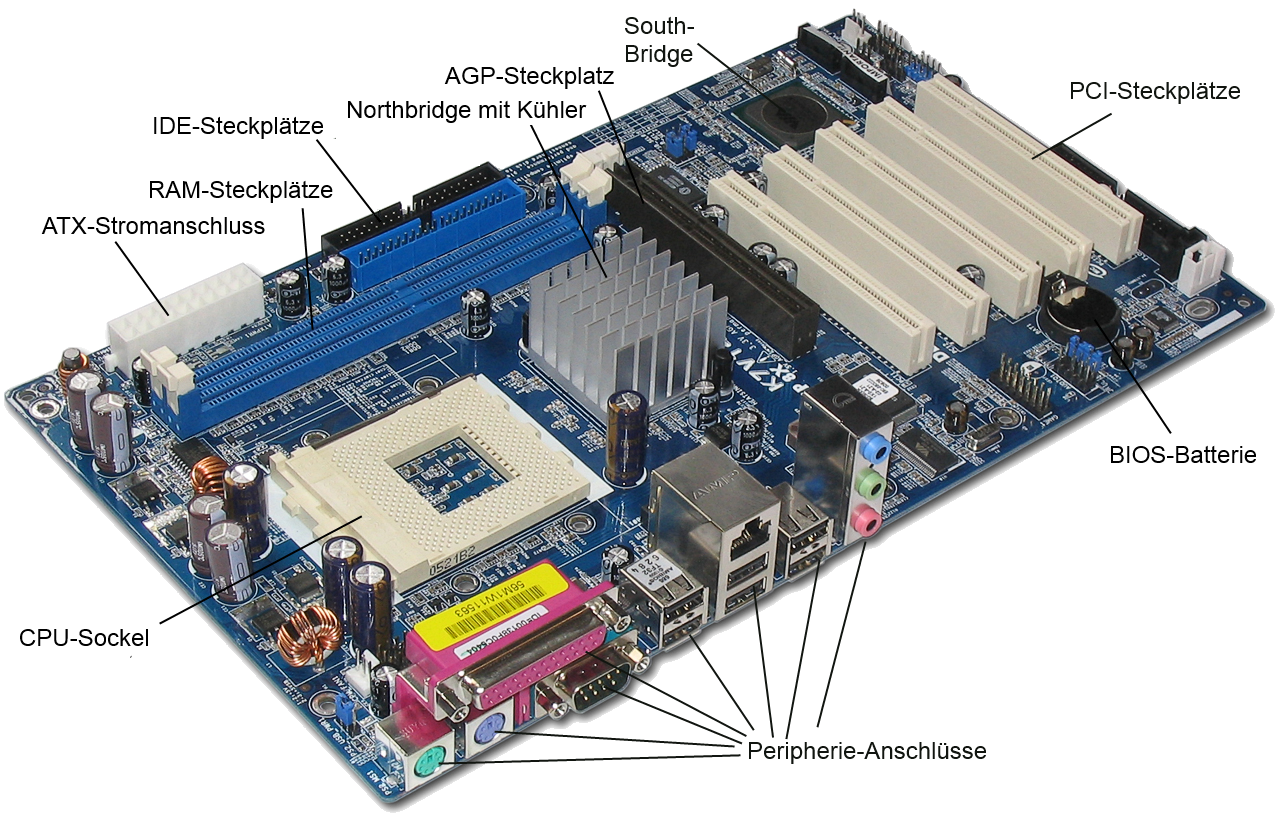
\includegraphics[width=1\textwidth]{motherboard}
  \caption{Motherboard}
  \end{figure}
  \end{column}
  \end{columns}
\end{frame}


\begin{frame}\frametitle{What do we need?}
  \centering
  Numbers!
  \begin{figure}
  
\includegraphics[width=0.7\textwidth]{numbers}

  \end{figure}

\end{frame}

\begin{frame}\frametitle{Now what do we do with it?}
  \begin{columns}
  \begin{column}{6cm}
  \begin{figure}
  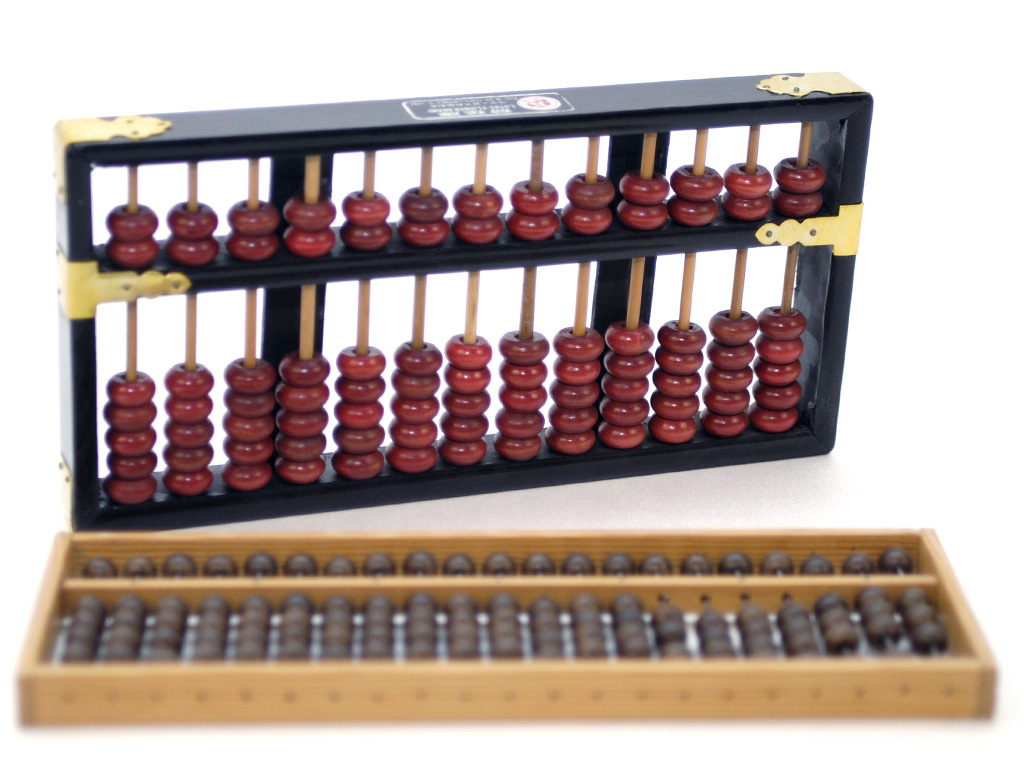
\includegraphics[width=1\textwidth]{abakus}
  \caption{Calculations}
  \end{figure}
  %\vspace{3cm} 
  \end{column}
  \begin{column}{6cm}
  \begin{figure}
  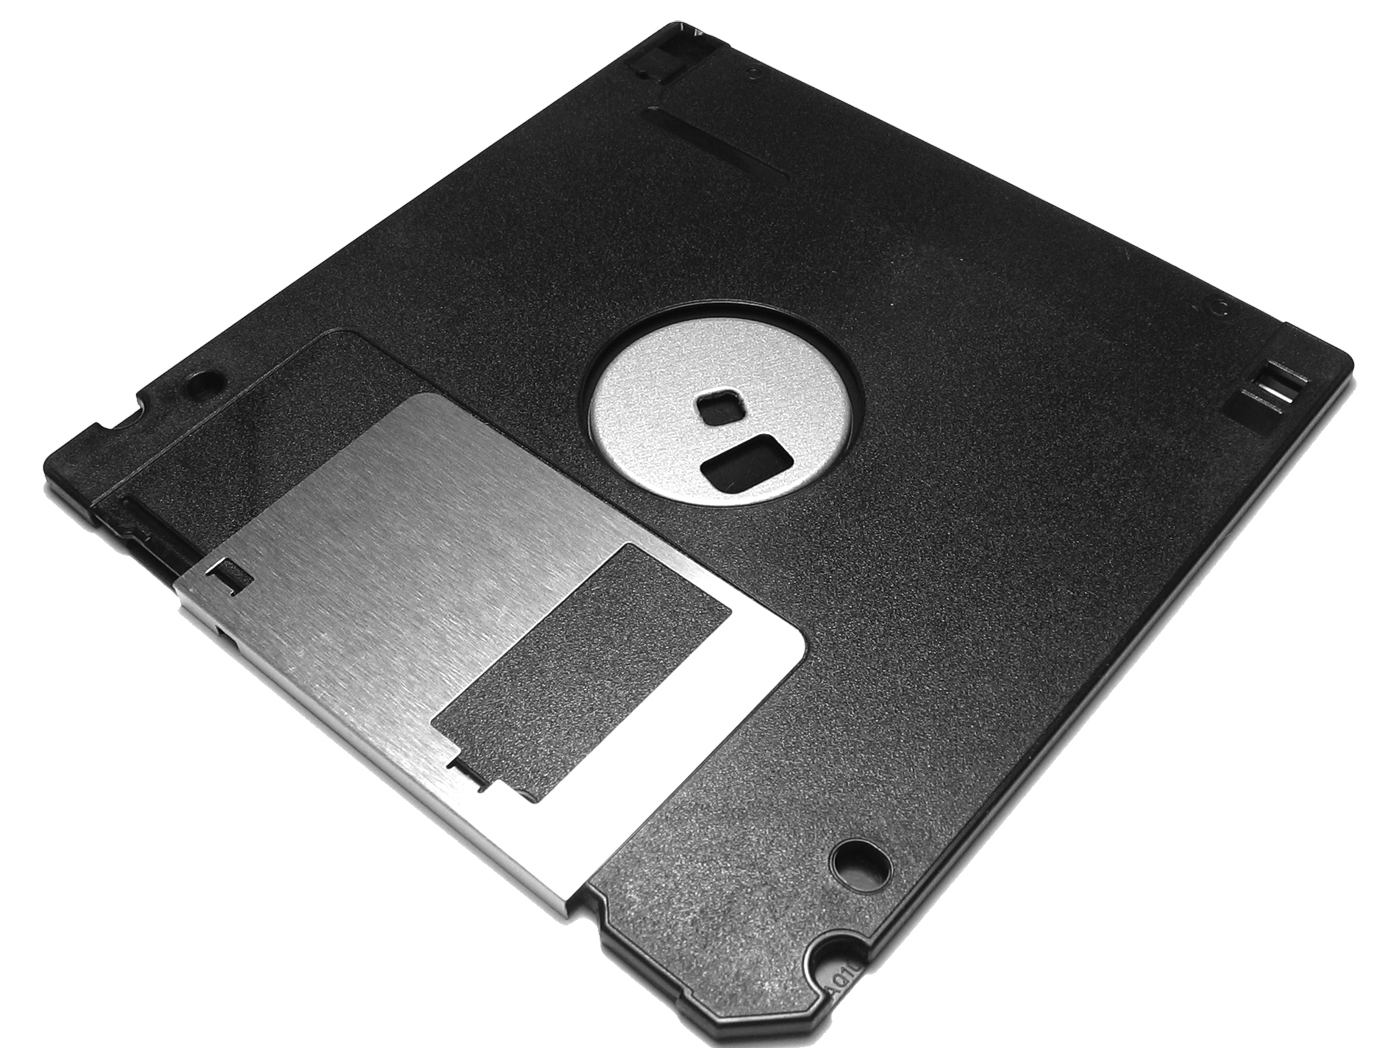
\includegraphics[width=1\textwidth]{memory}
  \caption{Memory}
  \end{figure}
  \end{column}
  \end{columns}
\end{frame}


\begin{frame}\frametitle{Now what do we do with it?}
  \begin{columns}
  \begin{column}{6cm}
  \begin{itemize}
   \item A computer is (most often) an electrical circuit
   \item Circuit should be able to calculate numbers and save them somehow
  \end{itemize}


  \end{column}
  \begin{column}{6cm}
  \begin{figure}
  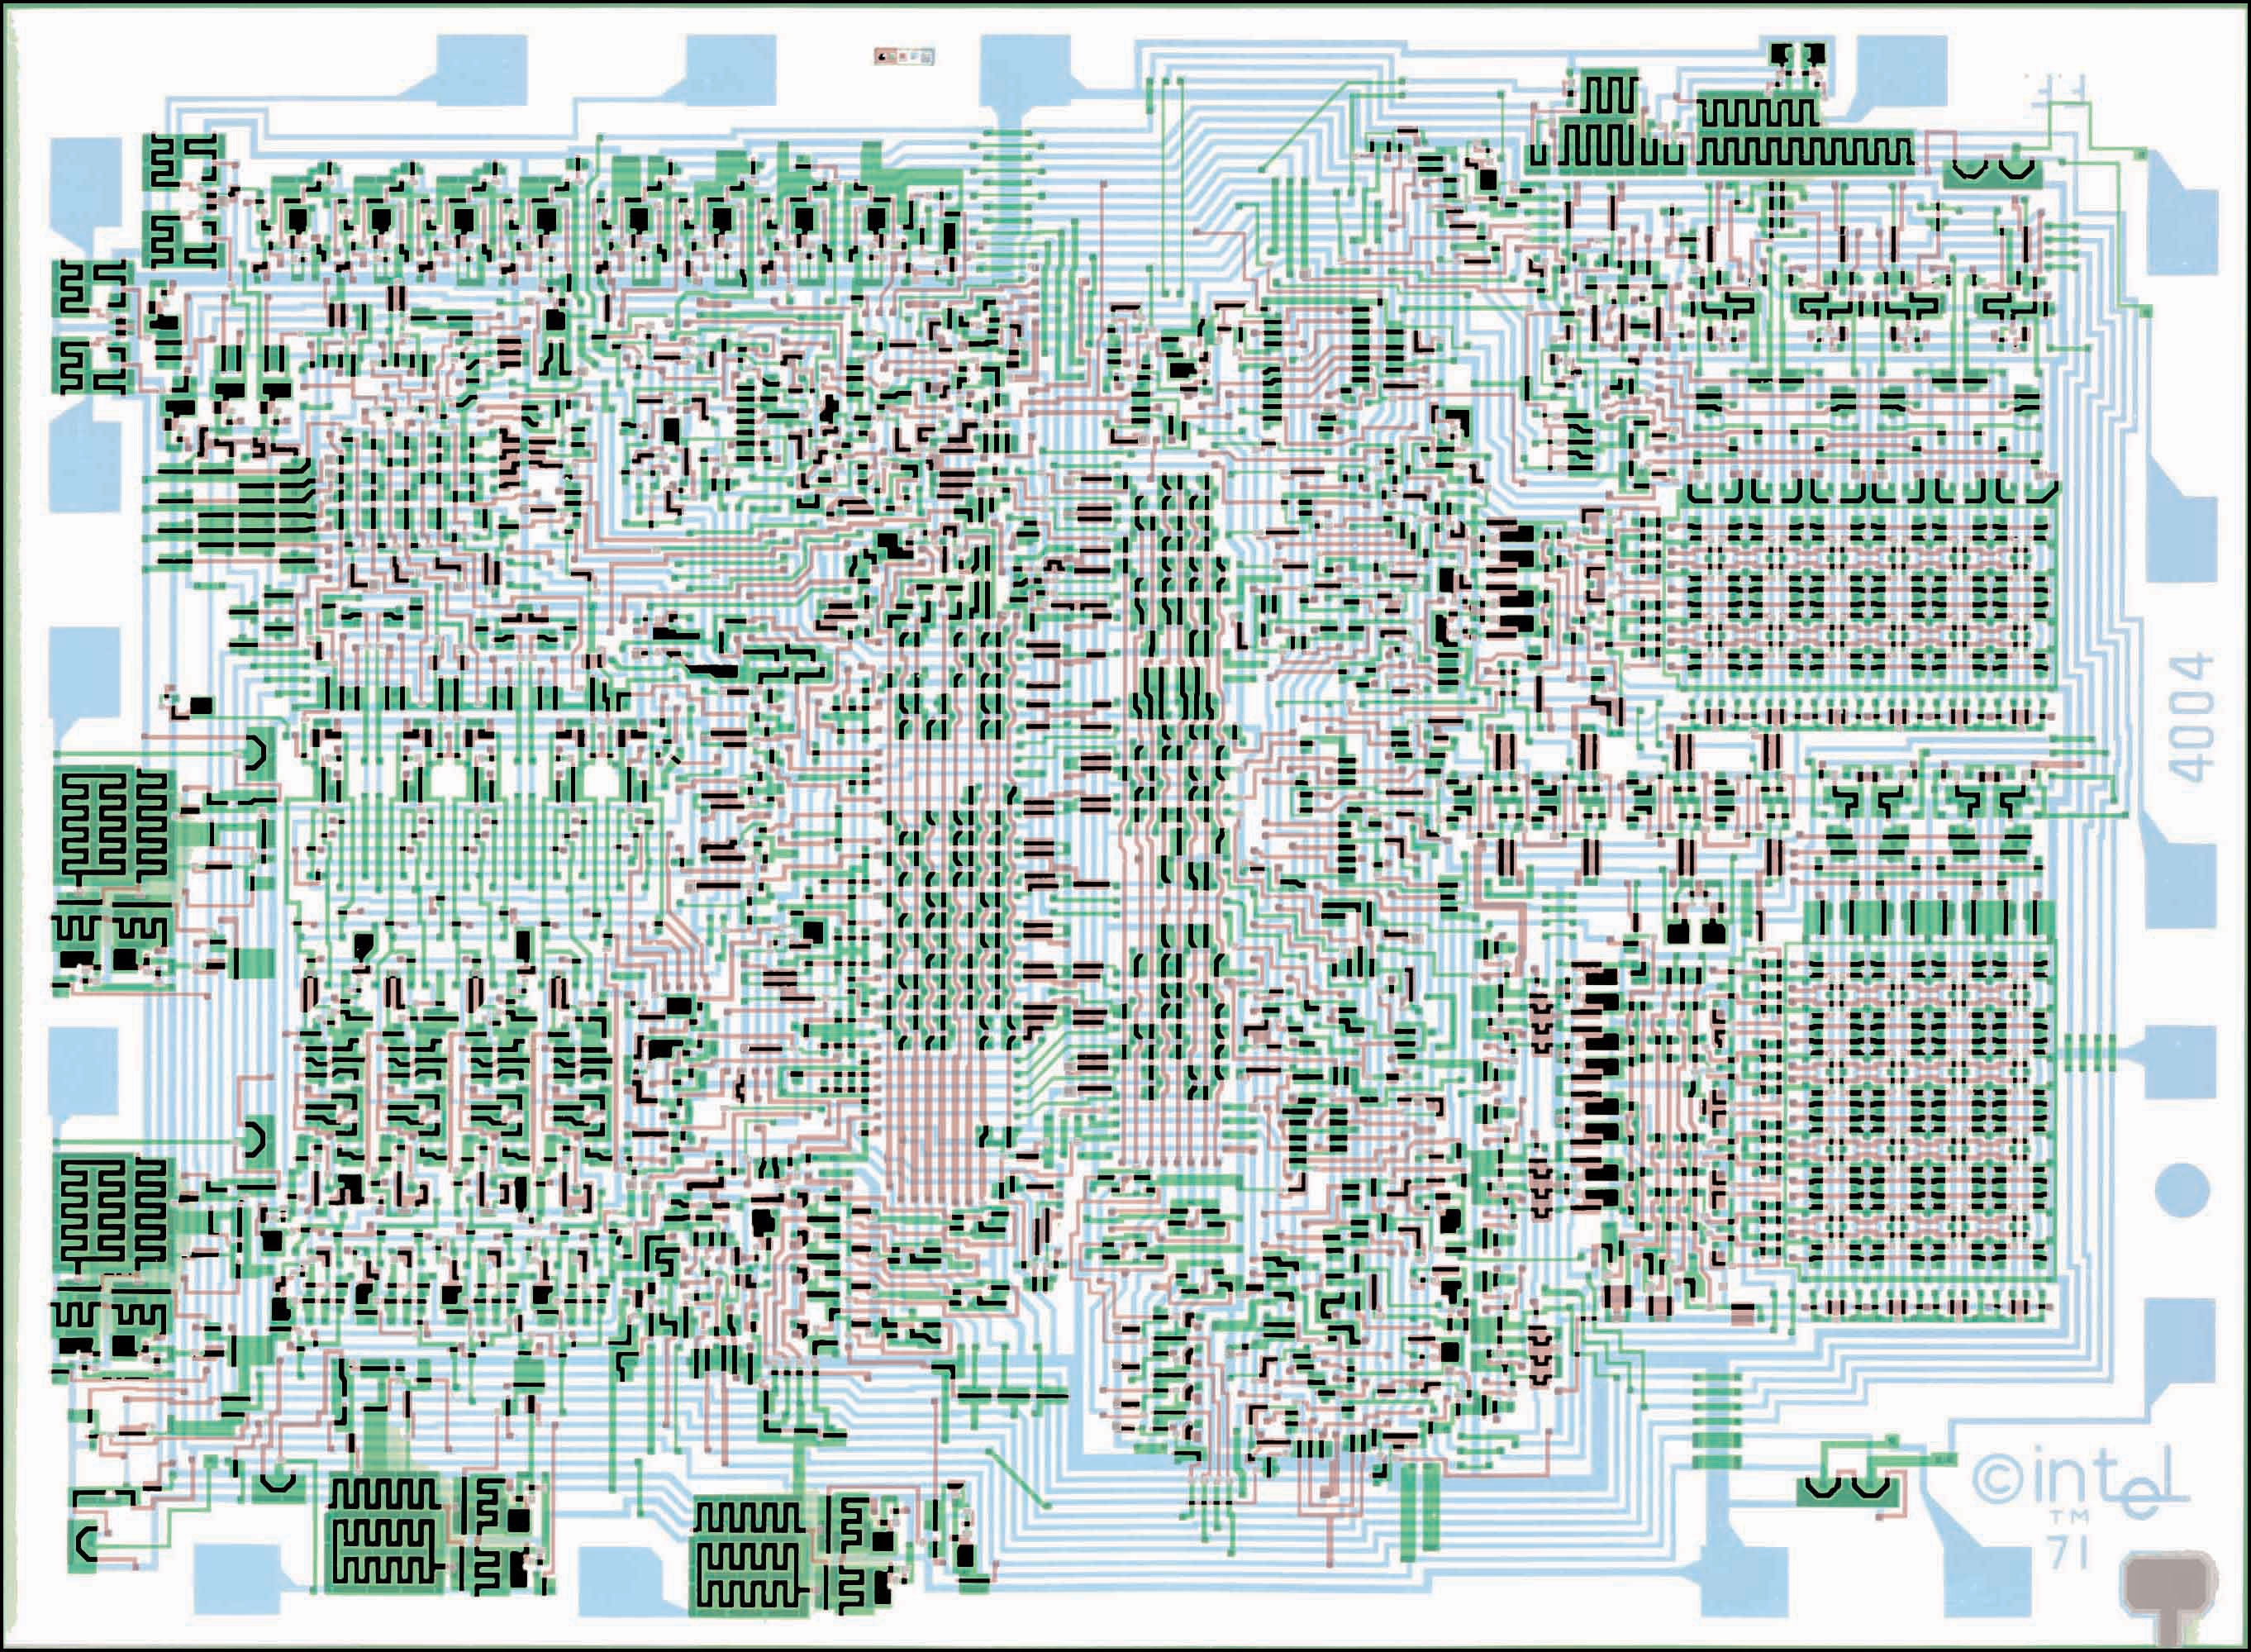
\includegraphics[width=0.9\textwidth]{4004}
  \caption{Intel 4004 Processor}
  \end{figure}
  \end{column}
  \end{columns}
\end{frame}

\section{Theory}
\frame{\tableofcontents[currentsection]}


\subsection{Digital Circuits}
\begin{frame}\frametitle{Analog Circuit}
  \begin{columns}
  \begin{column}{6cm}
  \begin{itemize}
   \item Continuous Voltage Levels
   \item Kirchhoff Ciruit Law's
   \item Example: Guitar Amplifier

  \end{itemize}


  \end{column}
  \begin{column}{6cm}
  \begin{figure}
  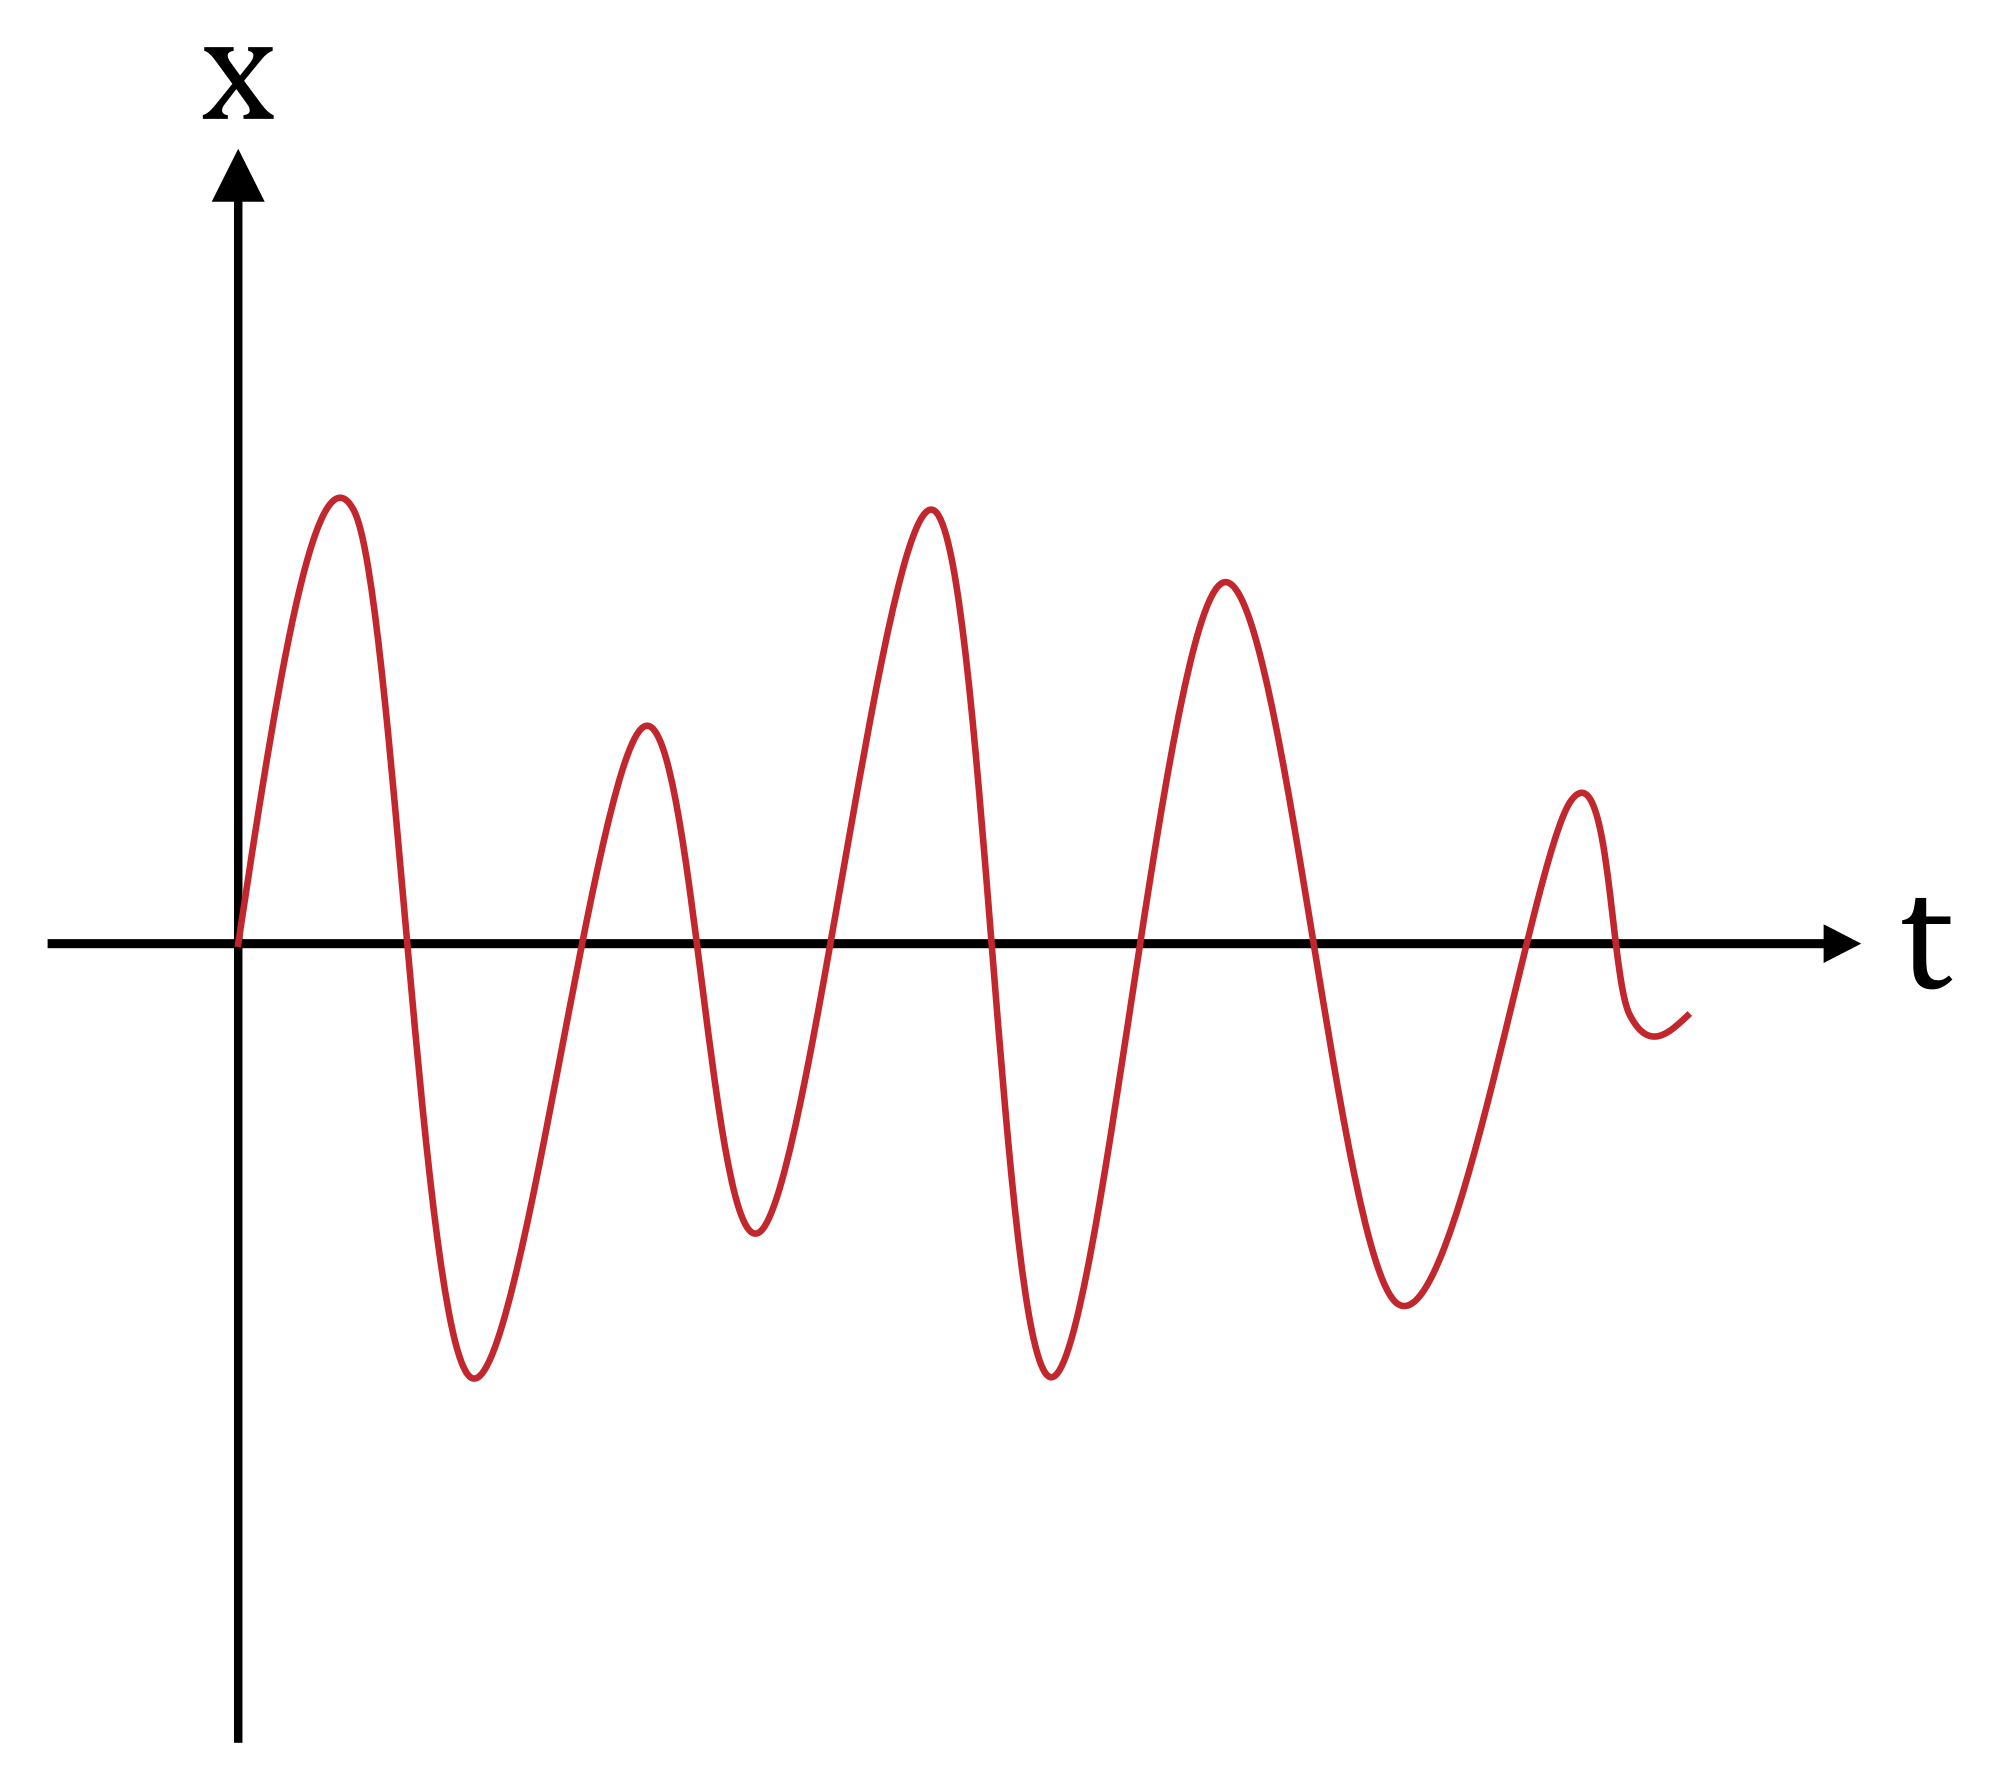
\includegraphics[width=0.9\textwidth]{analog}
  \caption{Analog Signal}
  \end{figure}
  \end{column}
  \end{columns}
\end{frame}

\begin{frame}\frametitle{Digital Circuit}
  \begin{columns}
  \begin{column}{6cm}
  \begin{itemize}
   \item Discrete Voltage Levels
   \item Is always based on an analog circuit.
   \item Example: Computer
   \item $\Rightarrow$ Binary Numbers

  \end{itemize}


  \end{column}
  \begin{column}{6cm}
  \begin{figure}
  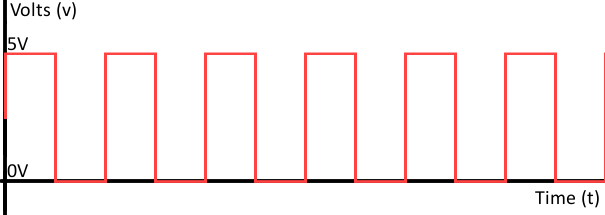
\includegraphics[width=1\textwidth]{digital}
  \caption{Digital Signal}
  \end{figure}
  \end{column}
  \end{columns}
\end{frame}


\subsection{Binary Numbers}
\begin{frame}\frametitle{Binary Numbers}
  \begin{columns}
  \begin{column}{6cm}
  \begin{itemize}
   \item<1-> High Voltage = 1
   \item<1-> Low Voltage = 0
   \item<1-> Can represent anything from numbers over letters to mp4 videos.
   \item 
  \end{itemize}

  \end{column}
  \begin{column}{6cm}
%   \begin{figure}
%   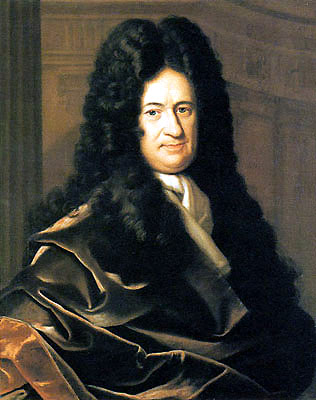
\includegraphics[height=0.6\textheight]{leibniz}
%   \caption{Gottfried Leibniz, 1679}
%   \end{figure}
  \end{column}
  \end{columns}
\end{frame}

\begin{frame}\frametitle{Binary Numbers}
  \begin{columns}
  \begin{column}{6cm}
  \begin{itemize}
   \item High Voltage = 1
   \item Low Voltage = 0
   \item Can represent anything from numbers over letters to mp4 videos.
   \item Binary System was invented in 1679 by Leibniz
  \end{itemize}

  \end{column}
  \begin{column}{6cm}
  \begin{figure}
  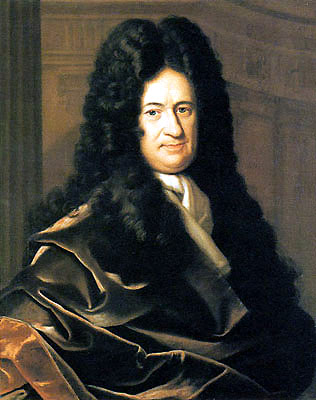
\includegraphics[height=0.6\textheight]{leibniz}
  \caption{Gottfried Leibniz, 1679}
  \end{figure}
  \end{column}
  \end{columns}
\end{frame}


\begin{frame}\frametitle{Binary Numbers}
  \begin{figure}
  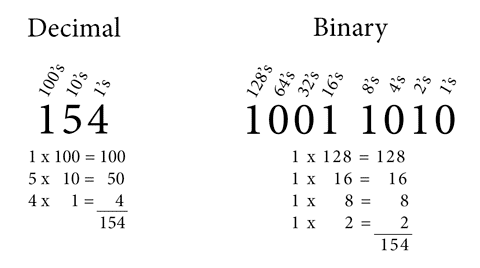
\includegraphics[width=0.8\textwidth]{dec_vs_bin}
  \caption{Different number representations}
  \end{figure}
\end{frame}


\subsection{Boolean Algebra}
\begin{frame}\frametitle{Boolean Algebra}
  \begin{columns}
  \begin{column}{6cm}
  \begin{itemize}
    \item<1-> \textbf{The conjunction (AND):} $a\land b$ is $1$ if and only if $a$ is $1$ and $b$ is $1$.\\
    \item<1->  \textbf{The disjunction (OR):} $a\lor b$  is $1$ if and only if $a$ is $1$ or $b$ is $1$ or both.\\
    \item<1->  \textbf{The negation (NOT):}  $\overline{a}$ is $1$ if and only if $a$ is $0$.
    \item<2->  Associative, Commutative, Distributive, Inverse, Zero
  \end{itemize}
  \end{column}
  
    
  \begin{column}{6cm}
  \begin{table}[H]
  \centering
  \begin{tabular}{c|c||c|c|c}
  \textbf{$a$} & \textbf{$b$} & \textbf{$a\land b$} & \textbf{$a\lor b$} & \textbf{$\overline{a}$} \\ \hline
  0          & 0          & 0            & 0            & 1           \\
  0          & 1          & 0            & 1            & 1           \\
  1          & 0          & 0            & 1            & 0           \\
  1          & 1          & 1            & 1            & 0          
  \end{tabular}
  \caption{truth table}
  \label{tab:truth}
  \end{table}
  \end{column}
  
  \end{columns}
\end{frame}

\subsection{Truth Tables}
\begin{frame}\frametitle{Truth tables}
  \begin{table}[H]
  \centering
  \begin{tabular}{c|c||c|c|c}
  \textbf{$a$} & \textbf{$b$} & \textbf{$a\land b$} & \textbf{$a\lor b$} & \textbf{$\overline{a}$} \\ \hline
  0          & 0          & 0            & 0            & 1           \\
  0          & 1          & 0            & 1            & 1           \\
  1          & 0          & 0            & 1            & 0           \\
  1          & 1          & 1            & 1            & 0          
  \end{tabular}
  \caption{truth table}
  \label{tab:truth2}
  \end{table}
\end{frame}

\begin{frame}\frametitle{Truth tables}
   \begin{table}[H]
  \centering
  \begin{tabular}{c|c||c|c|c|c|c}
  \textbf{$a$} & \textbf{$b$} & \textbf{$a\land b$} & \textbf{$a\lor b$} & \textbf{$\overline{a}$} & \textbf{ \textcolor{red}{$a==b$}}  & \textbf{ \textcolor{red}{$\overline{a\land  b}\ $}} \\ \hline
  0          & 0          & 0            & 0            & 1          & 1        & 1      \\
  0          & 1          & 0            & 1            & 1          & 0        & 1  \\
  1          & 0          & 0            & 1            & 0          & 0        & 1   \\
  1          & 1          & 1            & 1            & 0          & 1        & 0  
  \end{tabular}
  \caption{truth table}
  \label{tab:truth3}
  \end{table}
\end{frame}



\subsection{Disjunctive Normal-Form}
\begin{frame}\frametitle{Disjunctive Normal-Form}
  
  \begin{columns}
  \begin{column}{6cm}
  \begin{itemize}
    \item Let's convert this table in one compact formula!
    \item Disjunctive Normal Form:
    \begin{enumerate}
     \item \textbf{Rows} with logical output \textbf{1}.
     \item Combine inputs with AND. Each row separatly.
     \item Combine rows with logical OR.
    \end{enumerate}
    \item Example 1: 
    \begin{itemize}
      \item [\textbf{AND:}]$(a\land b)$
    \end{itemize}
  \end{itemize}
  \end{column}
  
    
  \begin{column}{6cm}
  \begin{table}[H]
  \centering
  \begin{tabular}{c|c||c}
  \textbf{$a$} & \textbf{$b$} & \textbf{$a\land b$} \\ \hline
  0          & 0          & 0      \\
  0          & 1          & 0  \\
  1          & 0          & 0   \\
  1          & 1          & 1 
  \end{tabular}
  \caption{truth table}
  \label{tab:truth4}
  \end{table}
  \end{column}
  
  \end{columns}  
\end{frame}


\begin{frame}\frametitle{Disjunctive Normal-Form}
  
  \begin{columns}
  \begin{column}{6cm}
  \begin{itemize}
    \item Let's convert this table in one compact formula!
    \item Disjunctive Normal Form:
    \begin{enumerate}
     \item \textbf{Rows} with logical output \textbf{1}.
     \item Combine inputs with AND. Each row separatly.
     \item Combine rows with logical OR.
    \end{enumerate}
    \item Example 2: 
    \begin{itemize}
      \item [\textbf{OR:}]$(\overline{a}\land b)\lor(a\land \overline{b})\lor(a\land b)$
    \end{itemize}
  \end{itemize}
  \end{column}
  
    
  \begin{column}{6cm}
  \begin{table}[H]
  \centering
  \begin{tabular}{c|c||c}
  \textbf{$a$} & \textbf{$b$} & \textbf{$a\lor b$} \\ \hline
  0          & 0          & 0      \\
  0          & 1          & 1  \\
  1          & 0          & 1   \\
  1          & 1          & 1 
  \end{tabular}
  \caption{truth table}
  \label{tab:truth}
  \end{table}
  \end{column}
  
  \end{columns}  
  
  
  
\end{frame}


\begin{frame}\frametitle{Disjunctive Normal-Form}
  
  \begin{columns}
  \begin{column}{6cm}
  \begin{itemize}
    \item Let's convert this table in one compact formula!
    \item Disjunctive Normal Form:
    \begin{enumerate}
     \item \textbf{Rows} with logical output \textbf{1}.
     \item Combine inputs with AND. Each row separatly.
     \item Combine rows with logical OR.
    \end{enumerate}
    \item Example 3: 
    \begin{itemize}
      \item [\textbf{==:}]$(\overline{a}\land \overline{b})\lor(a\land b)$
    \end{itemize}
  \end{itemize}
  \end{column}
  
    
  \begin{column}{6cm}
  \begin{table}[H]
  \centering
  \begin{tabular}{c|c||c}
  \textbf{$a$} & \textbf{$b$} & \textbf{$a == b$} \\ \hline
  0          & 0          & 1      \\
  0          & 1          & 0  \\
  1          & 0          & 0   \\
  1          & 1          & 1 
  \end{tabular}
  \caption{truth table}
  \label{tab:truth}
  \end{table}
  \end{column}
  
  \end{columns}  
  
  
  
\end{frame}






\section{Drawing and building a circuit}
\frame{\tableofcontents[currentsection]}


\subsection{Drawing a circuit}

\begin{frame}\frametitle{Logic Gates}
  \begin{figure}[H]
\centering
  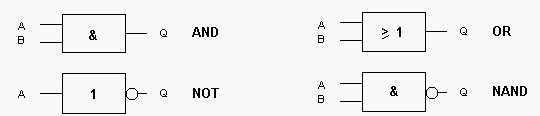
\includegraphics[width=0.8\textwidth]{gatter}%
  \caption{Logic circuit symbols}%
  \label{fig:logic_symbols}
\end{figure}
\end{frame}


\begin{frame}\frametitle{From Normal-Form to Circuit Diagram}
  \begin{columns}
  \begin{column}{5cm}
  Disjunctive normal-form for the equivalence: 
  \newline\newline
  $(a\land b)\lor(\overline{a}\land \overline{b})$
  \end{column}
  
  \begin{column}{6cm}
    \begin{figure}[H]
      \centering
      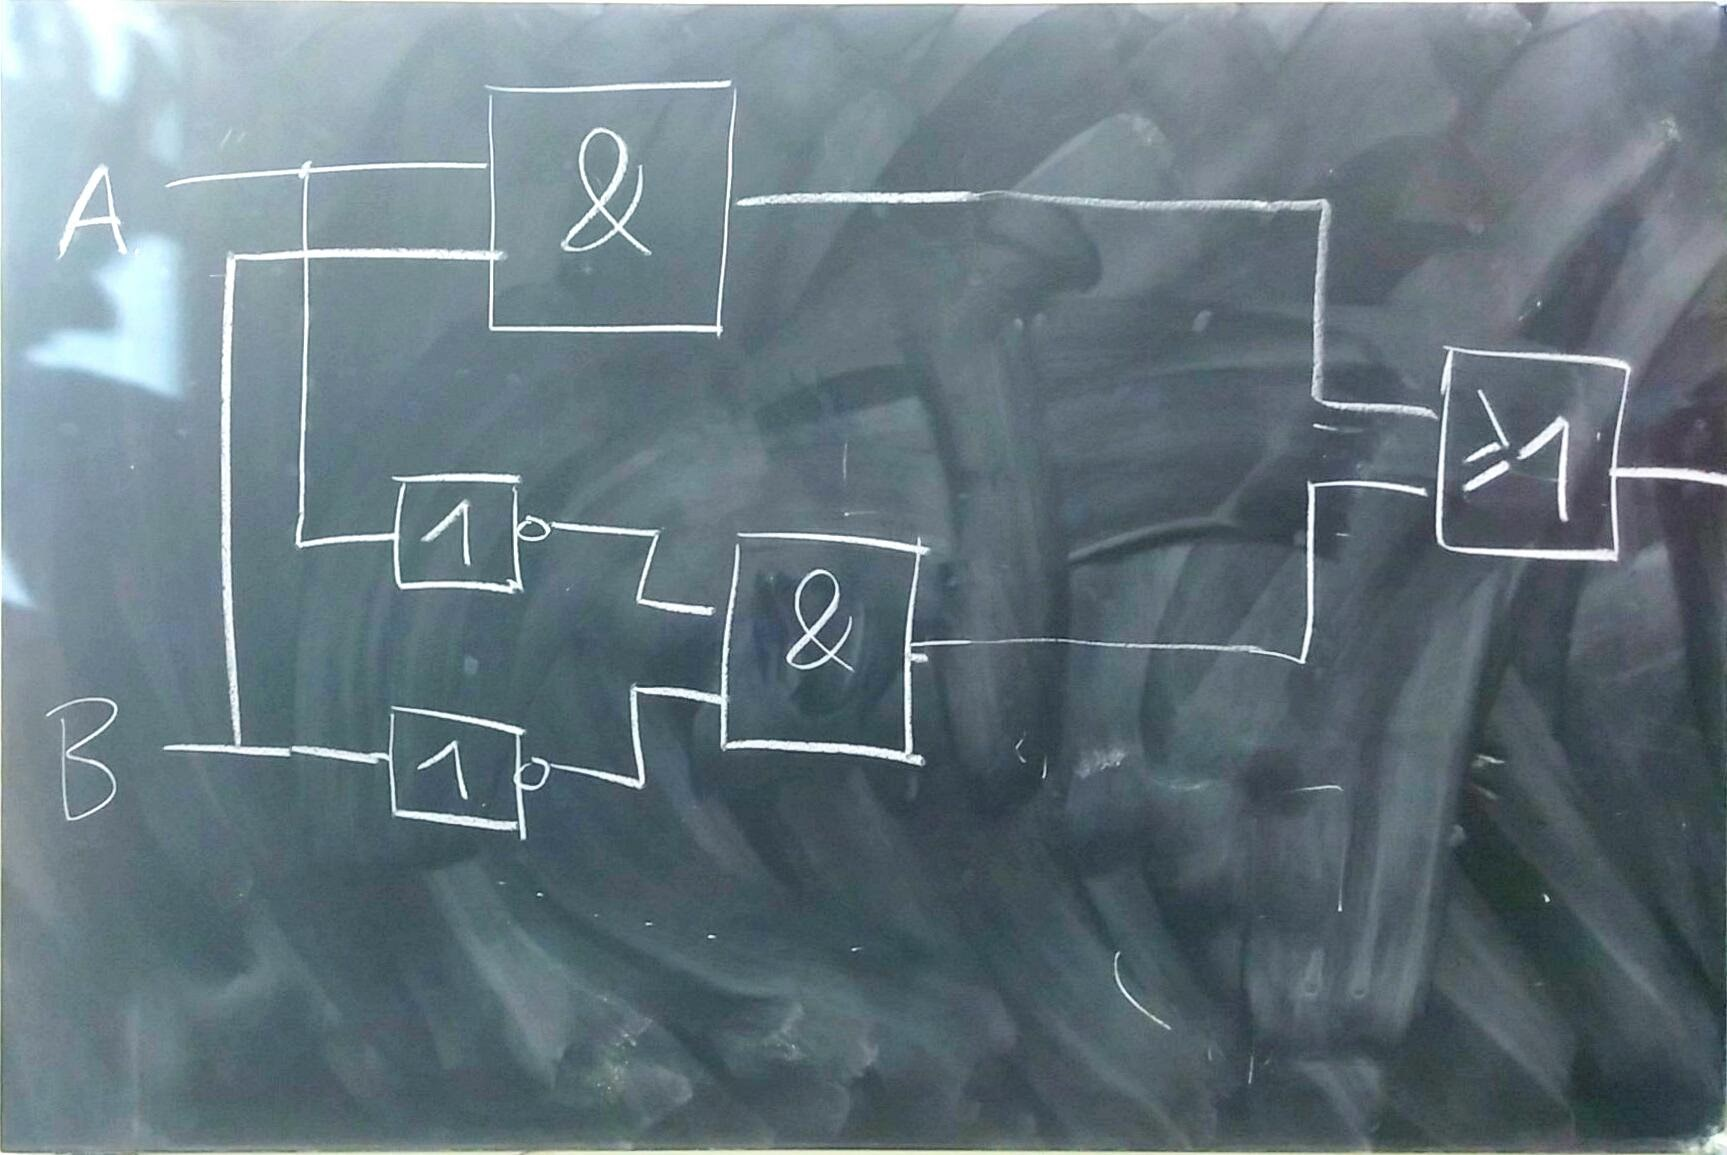
\includegraphics[width=1\textwidth]{eq1}%
      \caption{Example for circuit design: the equivalence}%
      \label{fig:equivalence}
    \end{figure}
  \end{column}
  \end{columns}  
\end{frame}


\begin{frame} \frametitle{NAND-Conversion}
  \begin{columns}
  \begin{column}{5cm}
  Now let's make it more complicated: \newline Use only NAND's! Why?
      \begin{figure}[H]
%       \centering
      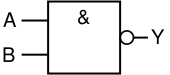
\includegraphics[width=0.35\textwidth]{nand}%
      \caption{NAND Gate}%
      \label{fig:nand}
    \end{figure}
  \begin{itemize}
   \item<2-> It's prettier
   \item<3-> For miniaturization, it's cheaper and more compact
  \end{itemize}

 % $(\overline{a}\land \overline{b})\lor(a\land b)$
  \end{column}
  
  \begin{column}{6cm}
    \begin{figure}[H]
      \centering
      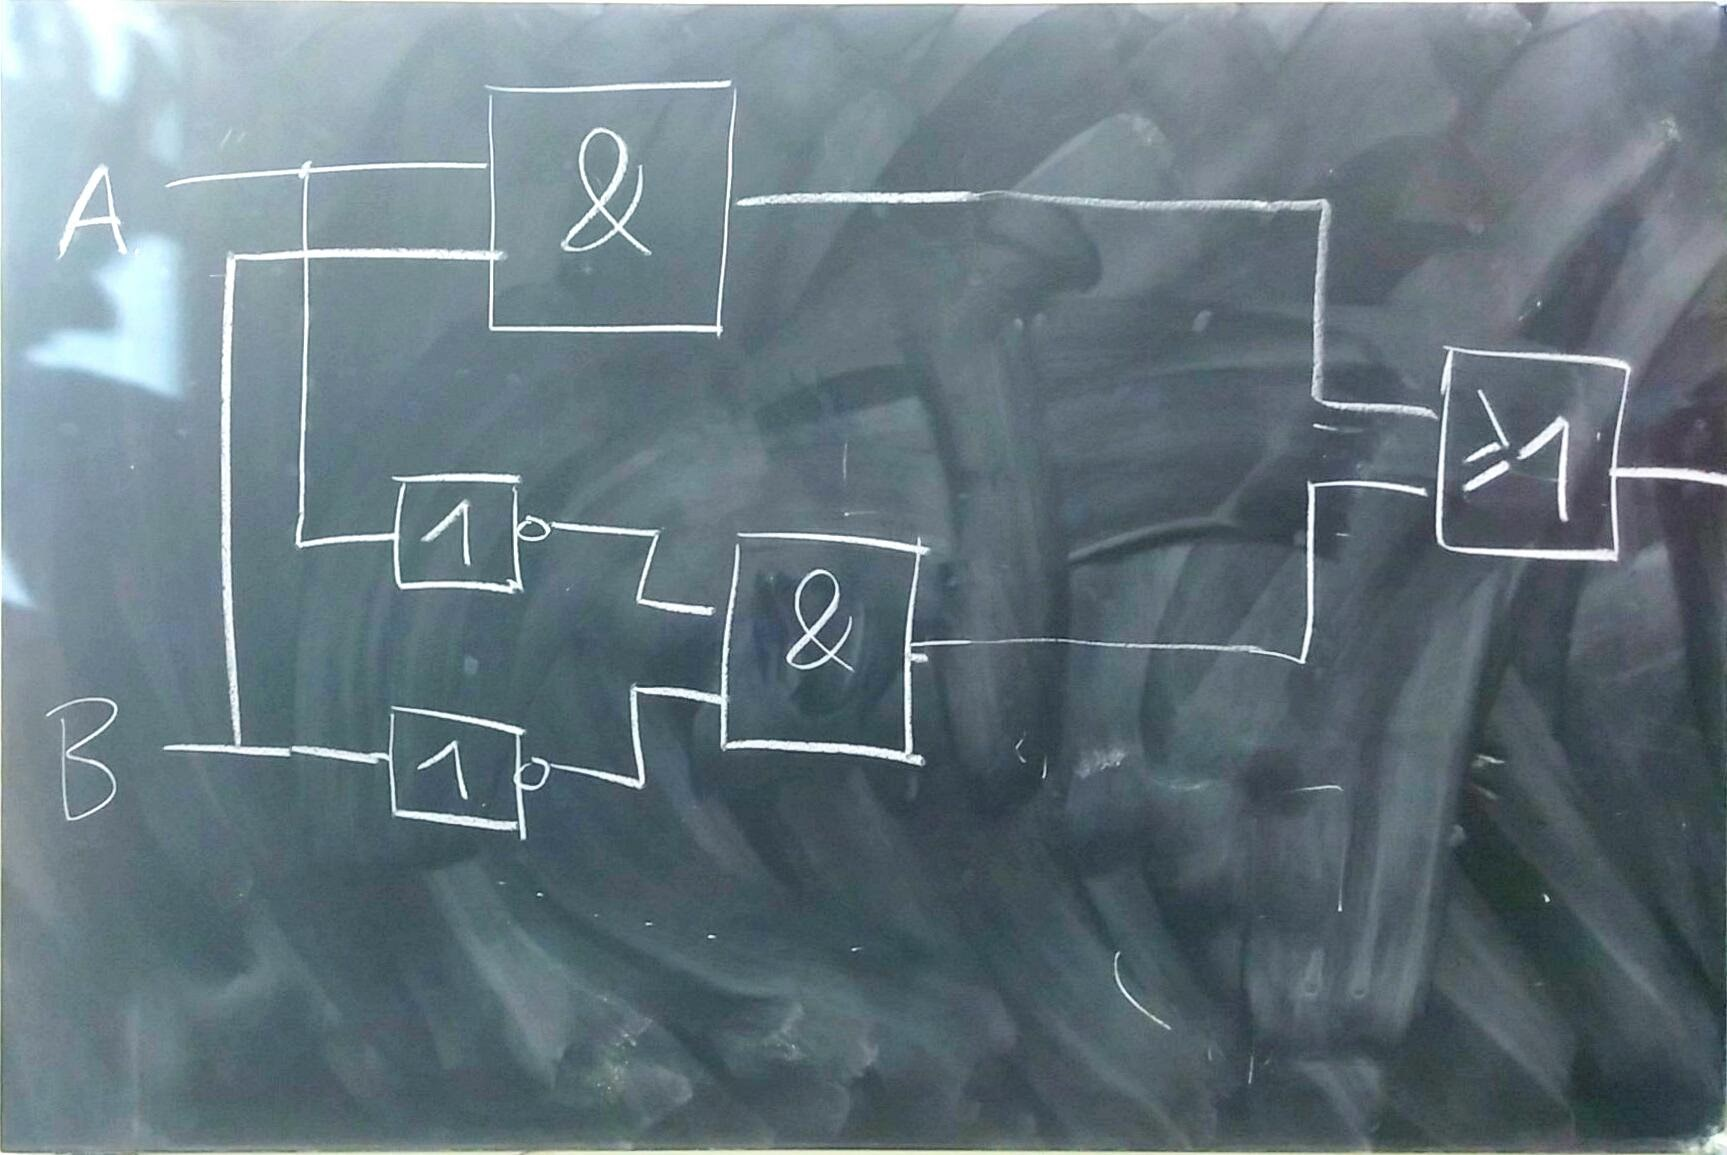
\includegraphics[width=1\textwidth]{eq1}%
      \caption{Optimized equivalence circuit}%
      \label{fig:equivalence_optimized}
    \end{figure}
  \end{column}
  \end{columns}  
\end{frame}


\begin{frame}  \frametitle{NAND-Conversion}
  \begin{columns}
  \begin{column}{5cm}
  Now let's make it more complicated: 
  \newline Use only NAND's! How?
  \newline\newline
  \pause Remember: Double inversion does not change anything! \newline $\overline{\overline{a}}=a$
 % $(\overline{a}\land \overline{b})\lor(a\land b)$
  \end{column}
  
  \begin{column}{6cm}
    \begin{figure}[H]
      \centering
      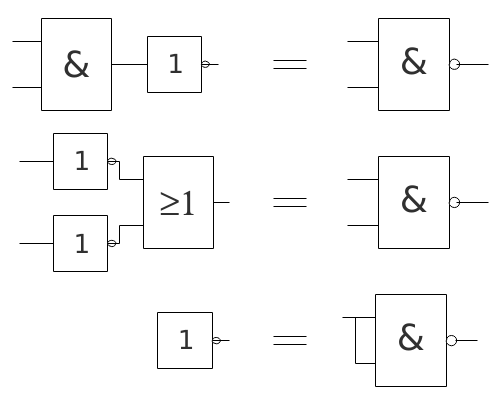
\includegraphics[width=1\textwidth]{nand_conversion}%
      \caption{NAND Conversion}%
      \label{fig:nand_conversion}
    \end{figure}
  \end{column}
  \end{columns}  
\end{frame}


\begin{frame}  \frametitle{NAND-Conversion}
  \begin{columns}
  \begin{column}{5cm}
  Use only NAND's! How?
  \newline
    \newline Example: Equivalence
  \newline
  $(\overline{a}\land \overline{b})\lor(a\land b)$
  \newline
  \begin{enumerate}
   \item Draw circuit as in disjunctive normal-form.
  \end{enumerate}

 % $(\overline{a}\land \overline{b})\lor(a\land b)$
  \end{column}
  
  \begin{column}{6cm}
    \begin{figure}[H]
      \centering
      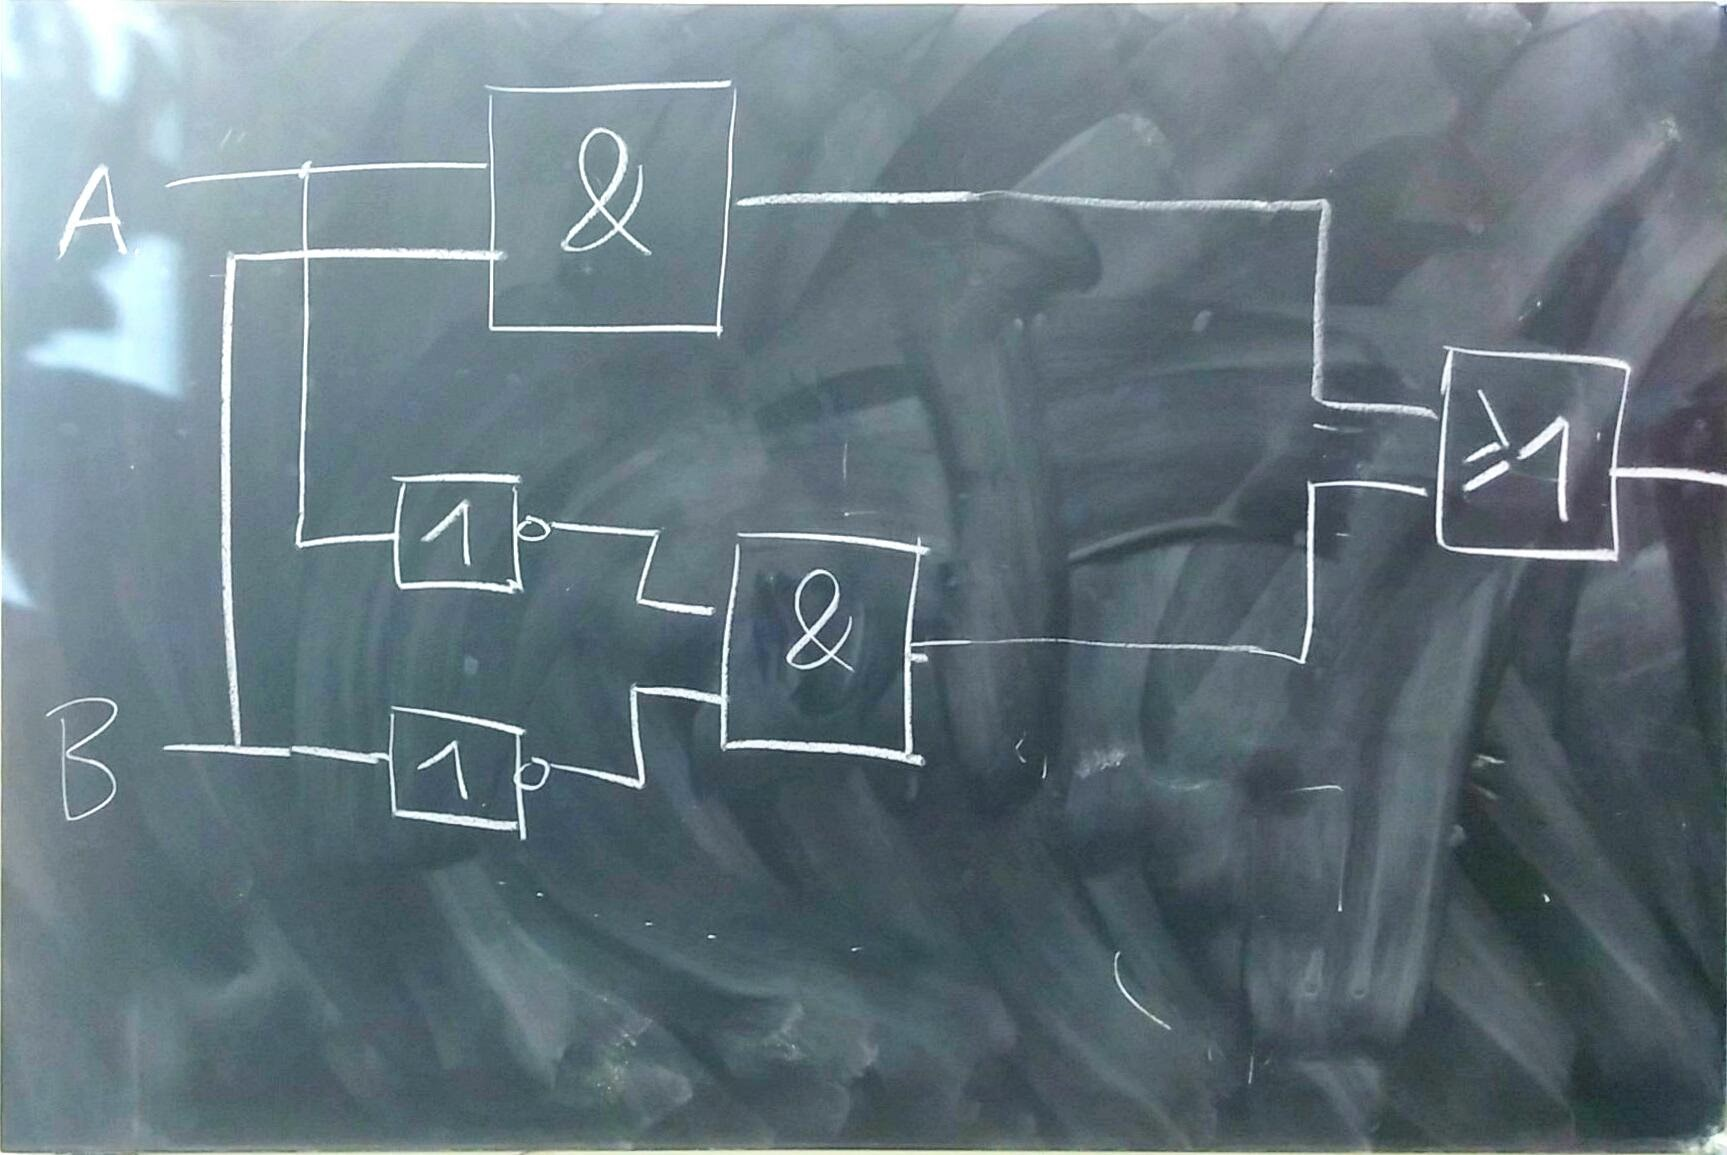
\includegraphics[width=1\textwidth]{eq1}%
      \caption{NAND Conversion}%
      \label{fig:eq1}
    \end{figure}
  \end{column}
  \end{columns}  
\end{frame}

\begin{frame}  \frametitle{NAND-Conversion}
  \begin{columns}
  \begin{column}{5cm}
  Use only NAND's! How?
    \newline Example: Equivalence
  \newline
  $(\overline{a}\land \overline{b})\lor(a\land b)$
  \newline
  \begin{enumerate}
   \item Draw circuit as in disjunctive normal-form.
   \item Plug in double inversions. See the patterns according to the conversion rules.
  \end{enumerate}

 % $(\overline{a}\land \overline{b})\lor(a\land b)$
  \end{column}
  
  \begin{column}{6cm}
    \begin{figure}[H]
      \centering
      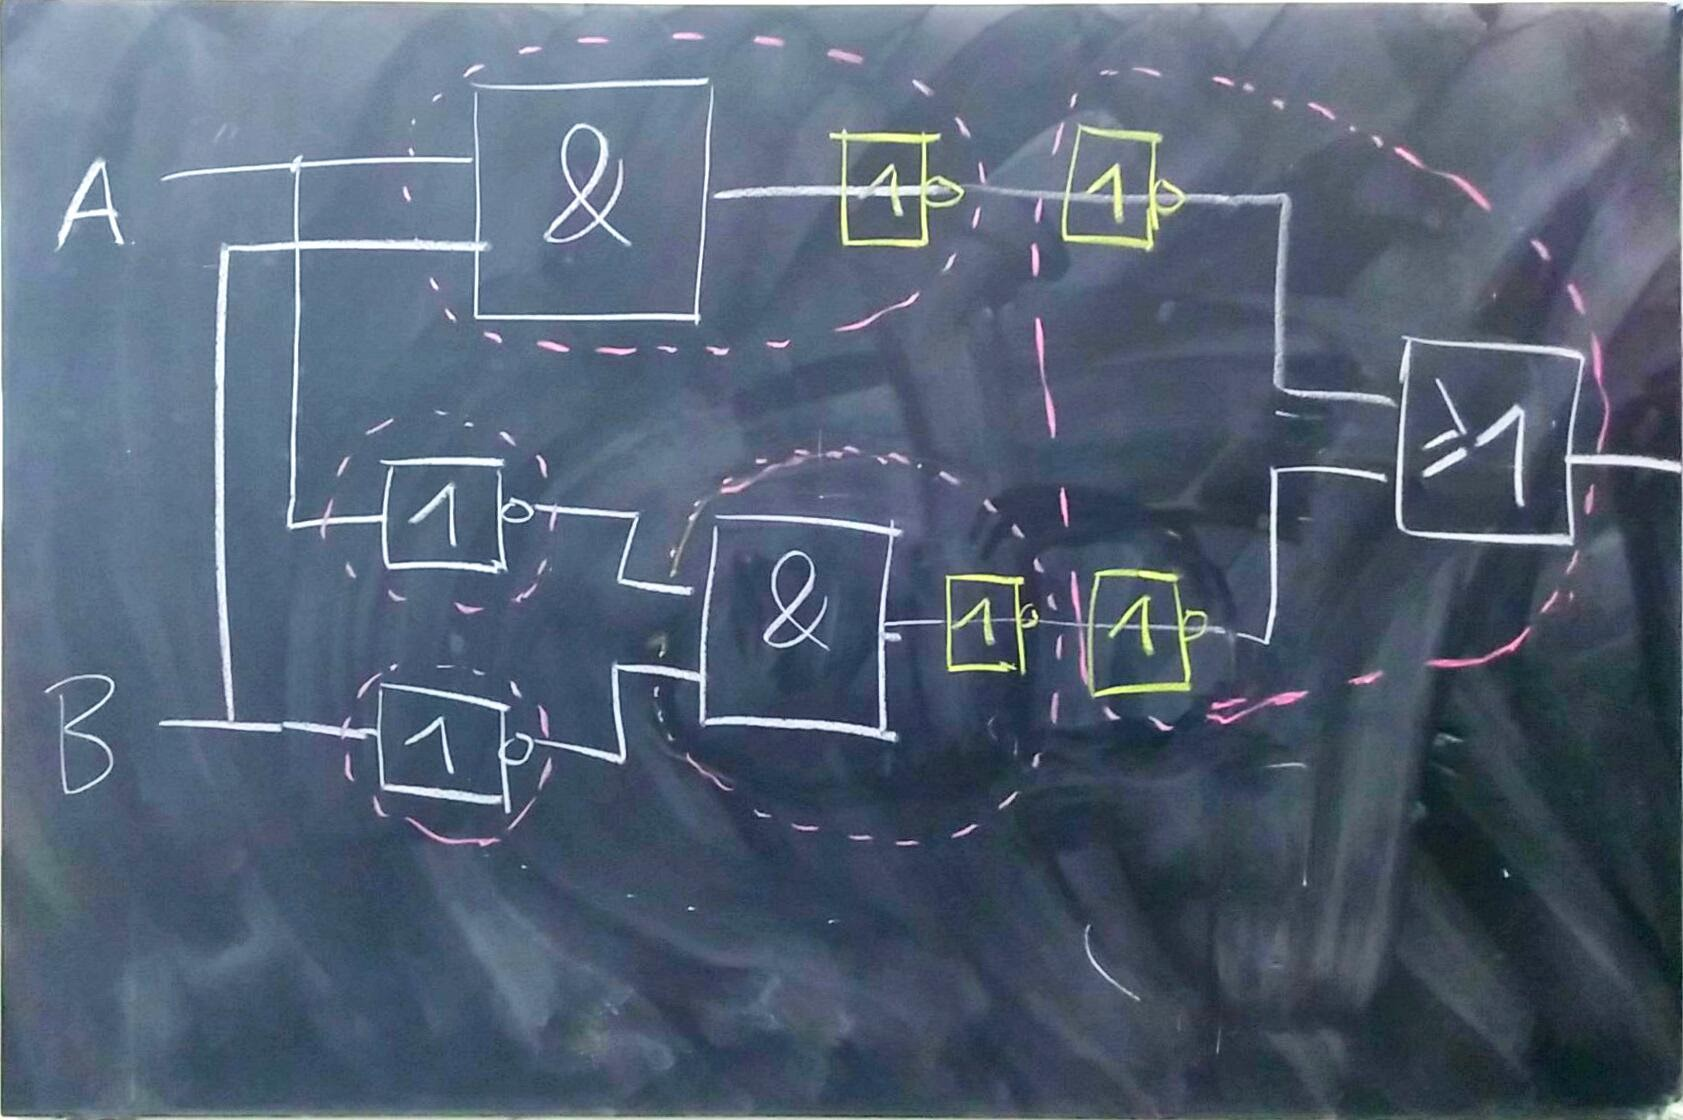
\includegraphics[width=1\textwidth]{eq2}%
      \caption{NAND Conversion}%
      \label{fig:eq2}
    \end{figure}
  \end{column}
  \end{columns}  
\end{frame}

\begin{frame}  \frametitle{NAND-Conversion}
  \begin{columns}
  \begin{column}{5cm}
  Use only NAND's! How?
    \newline Example: Equivalence
  \newline
  $(\overline{a}\land \overline{b})\lor(a\land b)$
  \newline
  \begin{enumerate}
   \item Draw circuit as in disjunctive normal-form.
   \item Plug in double inversions. See the patterns according to the conversion rules.
   \item Draw circuit again with NAND gates only.
  \end{enumerate}

 % $(\overline{a}\land \overline{b})\lor(a\land b)$
  \end{column}
  
  \begin{column}{6cm}
    \begin{figure}[H]
      \centering
      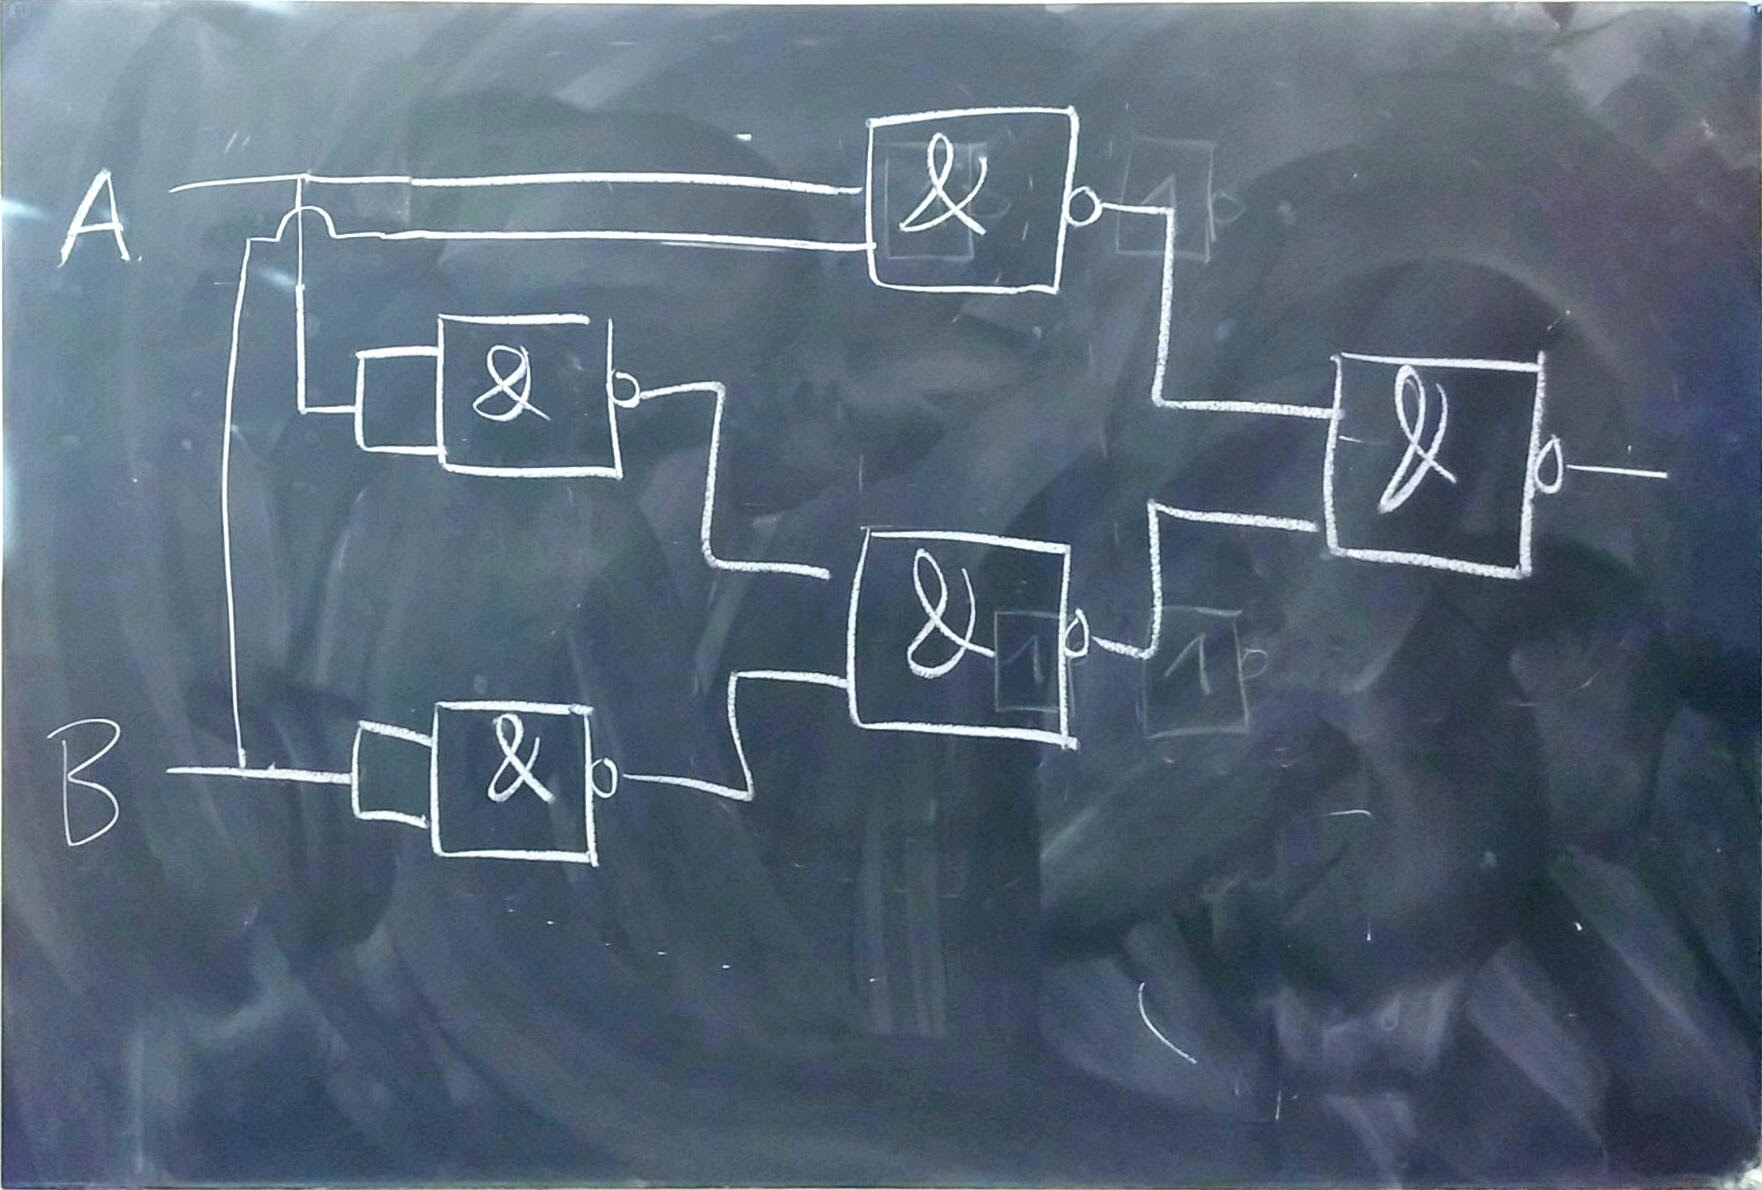
\includegraphics[width=1\textwidth]{eq3}%
      \caption{NAND Conversion}%
      \label{fig:eq3}
    \end{figure}
  \end{column}
  \end{columns}  
\end{frame}

\subsection{Building a circuit}
\begin{frame}  \frametitle{Building a circuit}
 Now we're ready to build the circuit with actual components!
 
\end{frame}

\begin{frame}  \frametitle{Breadboard}
Let's look at the breadboard design.
    \begin{figure}[H]
      \centering
      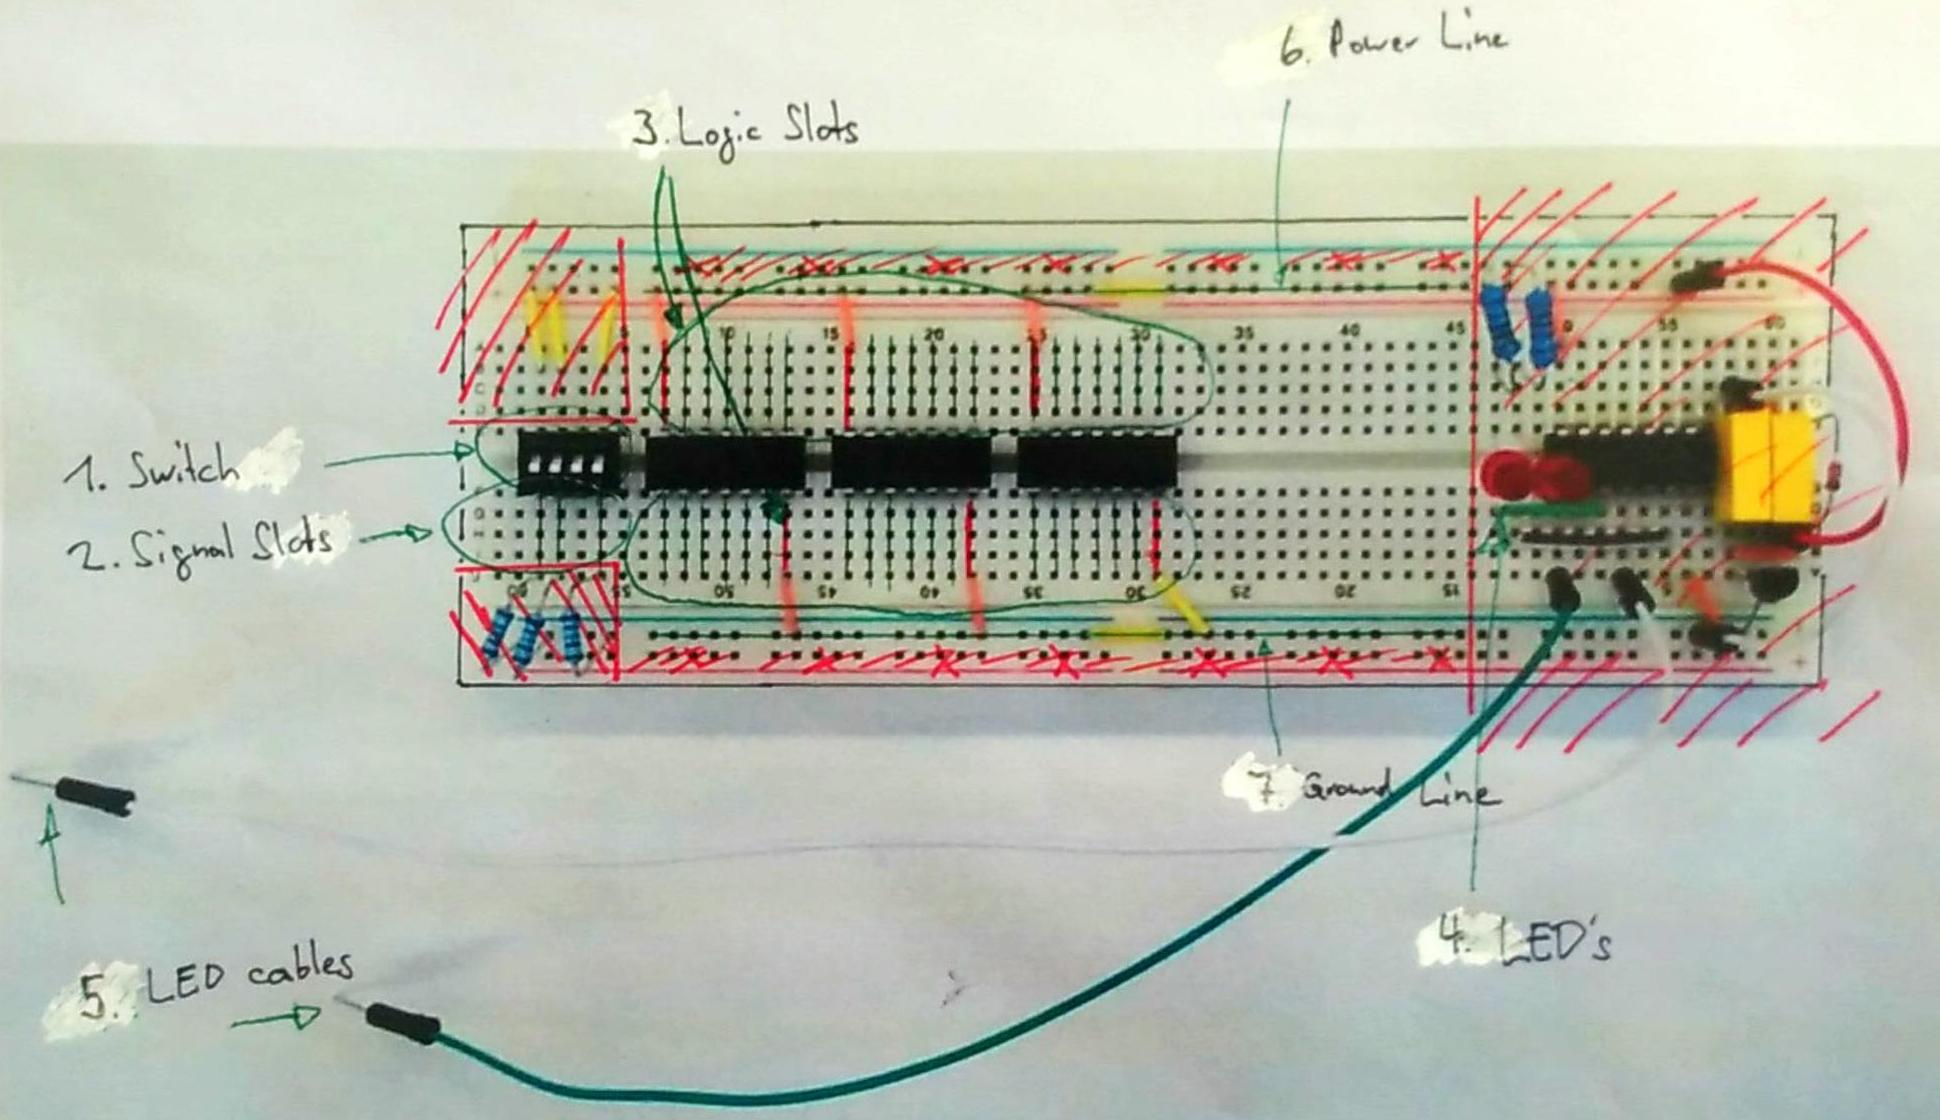
\includegraphics[width=0.9\textwidth]{breadboard_labeled}%
      \caption{Breadboard}%
      \label{fig:breadboard_labelled}
    \end{figure}
\end{frame}

\begin{frame}  \frametitle{Chip}
Now the chip design.
    \begin{figure}[H]
      \centering
      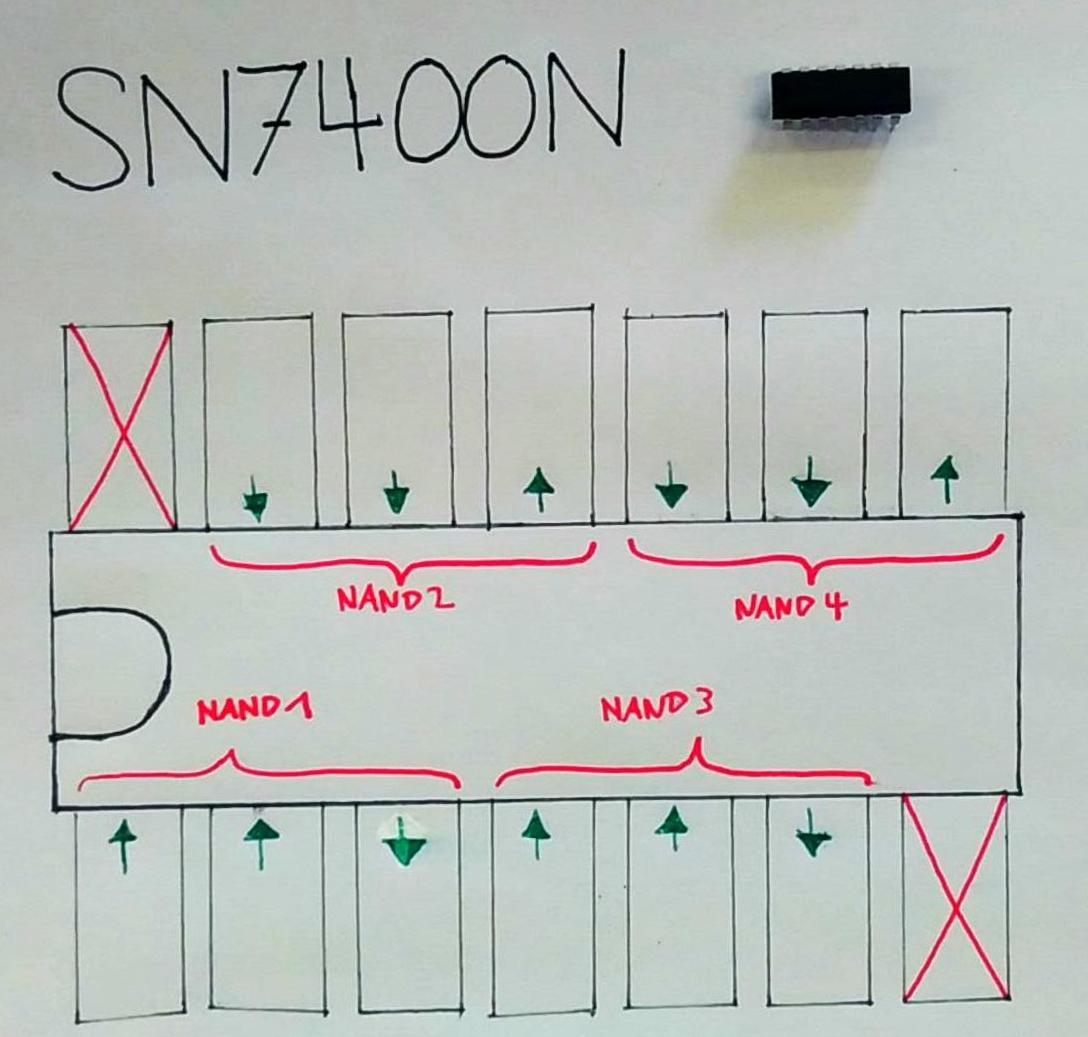
\includegraphics[width=0.5\textwidth]{sn7400n}%
      \caption{SN7400N Chip}%
      \label{fig:sn7400n}
    \end{figure}
\end{frame}

\begin{frame} \frametitle{Power Supply and Multimeter}
  \begin{columns}
  \begin{column}{6cm}
  \begin{figure}
  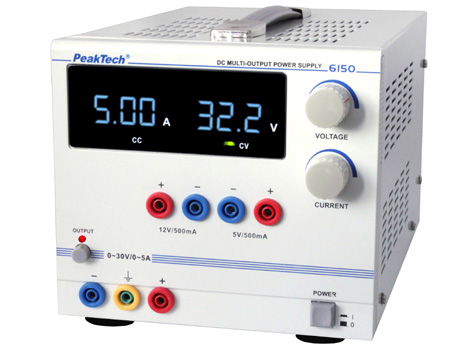
\includegraphics[width=0.8\textwidth]{power}
  \caption{Power Supply}
  \end{figure}
  %\vspace{3cm} 
  \end{column}
  \begin{column}{6cm}
  \begin{figure}
  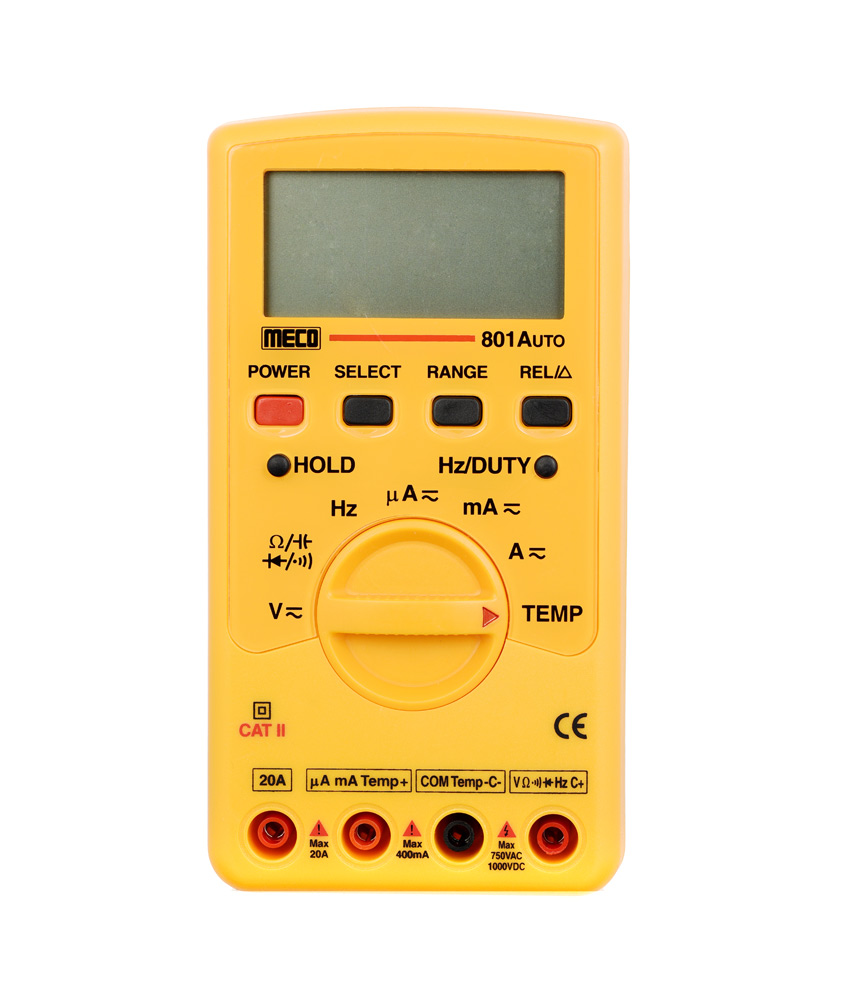
\includegraphics[width=0.7\textwidth]{multim}
  \caption{Multimeter}
  \end{figure}
  \end{column}
  \end{columns}
\end{frame}



\section{Sequential Circuits}
\frame{\tableofcontents[currentsection]}


\begin{frame}\frametitle{Combinatoric vs. Sequential Circuits}
\begin{itemize}
 \item Sequential Circuits have a memory
 \item Output of an operator is used again as one of the inputs
\end{itemize}

%Now we look at sequential circuits, which is different from the combinatoric circuit. Sequential circuits have something that can be looked at as a memory. The clue is, that the output of an operator is used again as one of the inputs. This means, that the circuit depends not only on combinatoric input variables, but also from the output of the step before. In this way, the functionality of a memory is realized. 
%\end{frame}

%\begin{frame}\frametitle{Loop}
\begin{figure}[H]
\centering
  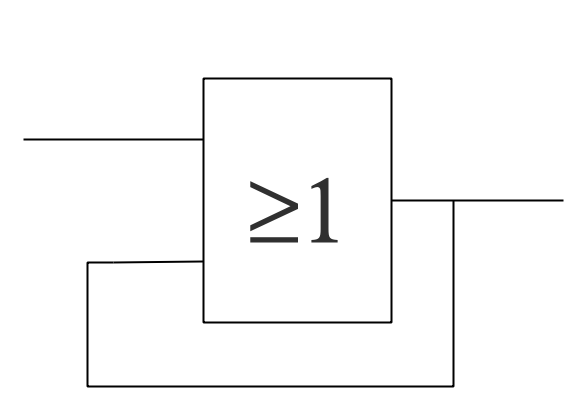
\includegraphics[width=0.4\textwidth]{loop}%
  \caption{Latch}%
  \label{fig:loop}
\end{figure}
\end{frame}

\begin{frame}\frametitle{RS-Flip-Flop}
\begin{figure}[H]
\centering
  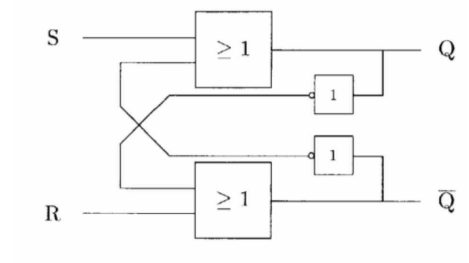
\includegraphics[width=0.7\textwidth]{RSFF}%
  \caption{RS-Flip-Flop}%
  \label{fig:RSFF}
\end{figure}
\end{frame}


\end{document}